\documentclass[11pt,a4paper]{article}
\usepackage[utf8]{inputenc}
\usepackage[T1]{fontenc}
\usepackage[polish]{babel}
\usepackage{amsmath, amsfonts, amssymb}
\usepackage{graphicx}
\usepackage[margin=2.5cm]{geometry}
\usepackage{float}
\usepackage{caption}
\usepackage{indentfirst}
\usepackage{hyperref}
\geometry{margin=2.5cm}
\title{Aproksymacja profilu wysokościowego\vspace{0.5em}\\Projekt 3 -- Metody Numeryczne}
\author{Yauheni Pyryeu 201253}
\date{\today}

\begin{document}
\maketitle
\thispagestyle{empty}
\newpage
\tableofcontents
\thispagestyle{empty}
\newpage
\setcounter{page}{1}

\section{Wstęp}
Profil wysokościowy trasy to wykres przedstawiający wysokość bezwzględną w terenie w zależności od odległości od początku trasy. Znając wysokość tylko części punktów trasy, możemy określić wysokości punktów pośrednich za pomocą aproksymacji interpolacyjnej. W projekcie zastosowano dwie metody interpolacji: wielomianową (Lagrange'a) oraz funkcje sklejane trzeciego stopnia (naturalne splajny kubiczne).

\section{Opis algorytmów}
\subsection{Interpolacja wielomianowa Lagrange'a}
Interpolacja polega na wyznaczeniu wielomianu przechodzącego przez zadane punkty (węzły). W celu poprawy stabilności numerycznej, przed wyznaczeniem wielomianu przekształcono dziedzinę do przedziału $[0,1]$.
\[ P(x) = \sum_{j=0}^{N-1} y_j L_j(x) \]
gdzie $L_j(x)$ to wielomiany bazowe Lagrange'a:
\[ L_j(x) = \prod_{m=0, m \neq j}^{N-1} \frac{x - x_m}{x_j - x_m} \]
Główną zaletą tej metody jest jej prostota koncepcyjna i gwarancja przejścia przez wszystkie węzły. Wadą jest podatność na tzw. zjawisko Rungego, czyli duże oscylacje wielomianu interpolacyjnego, szczególnie w pobliżu krańców przedziału, przy dużej liczbie równoodległych węzłów. W celu poprawy stabilności numerycznej obliczeń, dziedzina funkcji interpolowanej ($x_i$) jest przekształcana do przedziału $[0,1]$ przed wyznaczeniem wielomianu, a następnie wartości są transformowane z powrotem.

\subsection{Interpolacja funkcjami sklejanymi trzeciego stopnia}
Funkcje sklejane trzeciego stopnia (splajny kubiczne) to funkcje złożone z wielomianów trzeciego stopnia, definiowanych osobno na każdym podprzedziale $[x_i, x_{i+1}]$ pomiędzy kolejnymi węzłami. Każdy taki wielomian $S_i(x)$ jest tak dobrany, aby cała funkcja była ciągła oraz miała ciągłe pierwszą i drugą pochodną ($C^2$) w całym przedziale interpolacji. W przypadku naturalnych splajnów kubicznych dodatkowo wymaga się, aby drugie pochodne na końcach przedziału były równe zeru ($S''(x_0) = 0$, $S''(x_{N-1}) = 0$). Splajny kubiczne są mniej podatne na oscylacje niż wielomiany interpolacyjne wysokiego stopnia i zwykle zapewniają gładsze oraz bardziej realistyczne przybliżenie danych.

\section{Dane}
Do analizy wykorzystano rzeczywiste profile wysokościowe kilku tras o zróżnicowanym charakterze:
\begin{itemize}
    \item GdanskPromenade -- trasa prawie płaska,
    \item Hel -- trasa nadmorska,
    \item VariousHills -- trasa o wielu wzniesieniach,
    \item ChallengerDeep -- trasa z dużą różnicą wysokości.
\end{itemize}

\section{Analiza podstawowa interpolacji wielomianowej}
\subsection{Trasa: GdanskPromenade}
Wpływ liczby węzłów na jakość interpolacji Lagrange'a przedstawiono na rysunkach poniżej.

\begin{figure}[H]
    \centering
    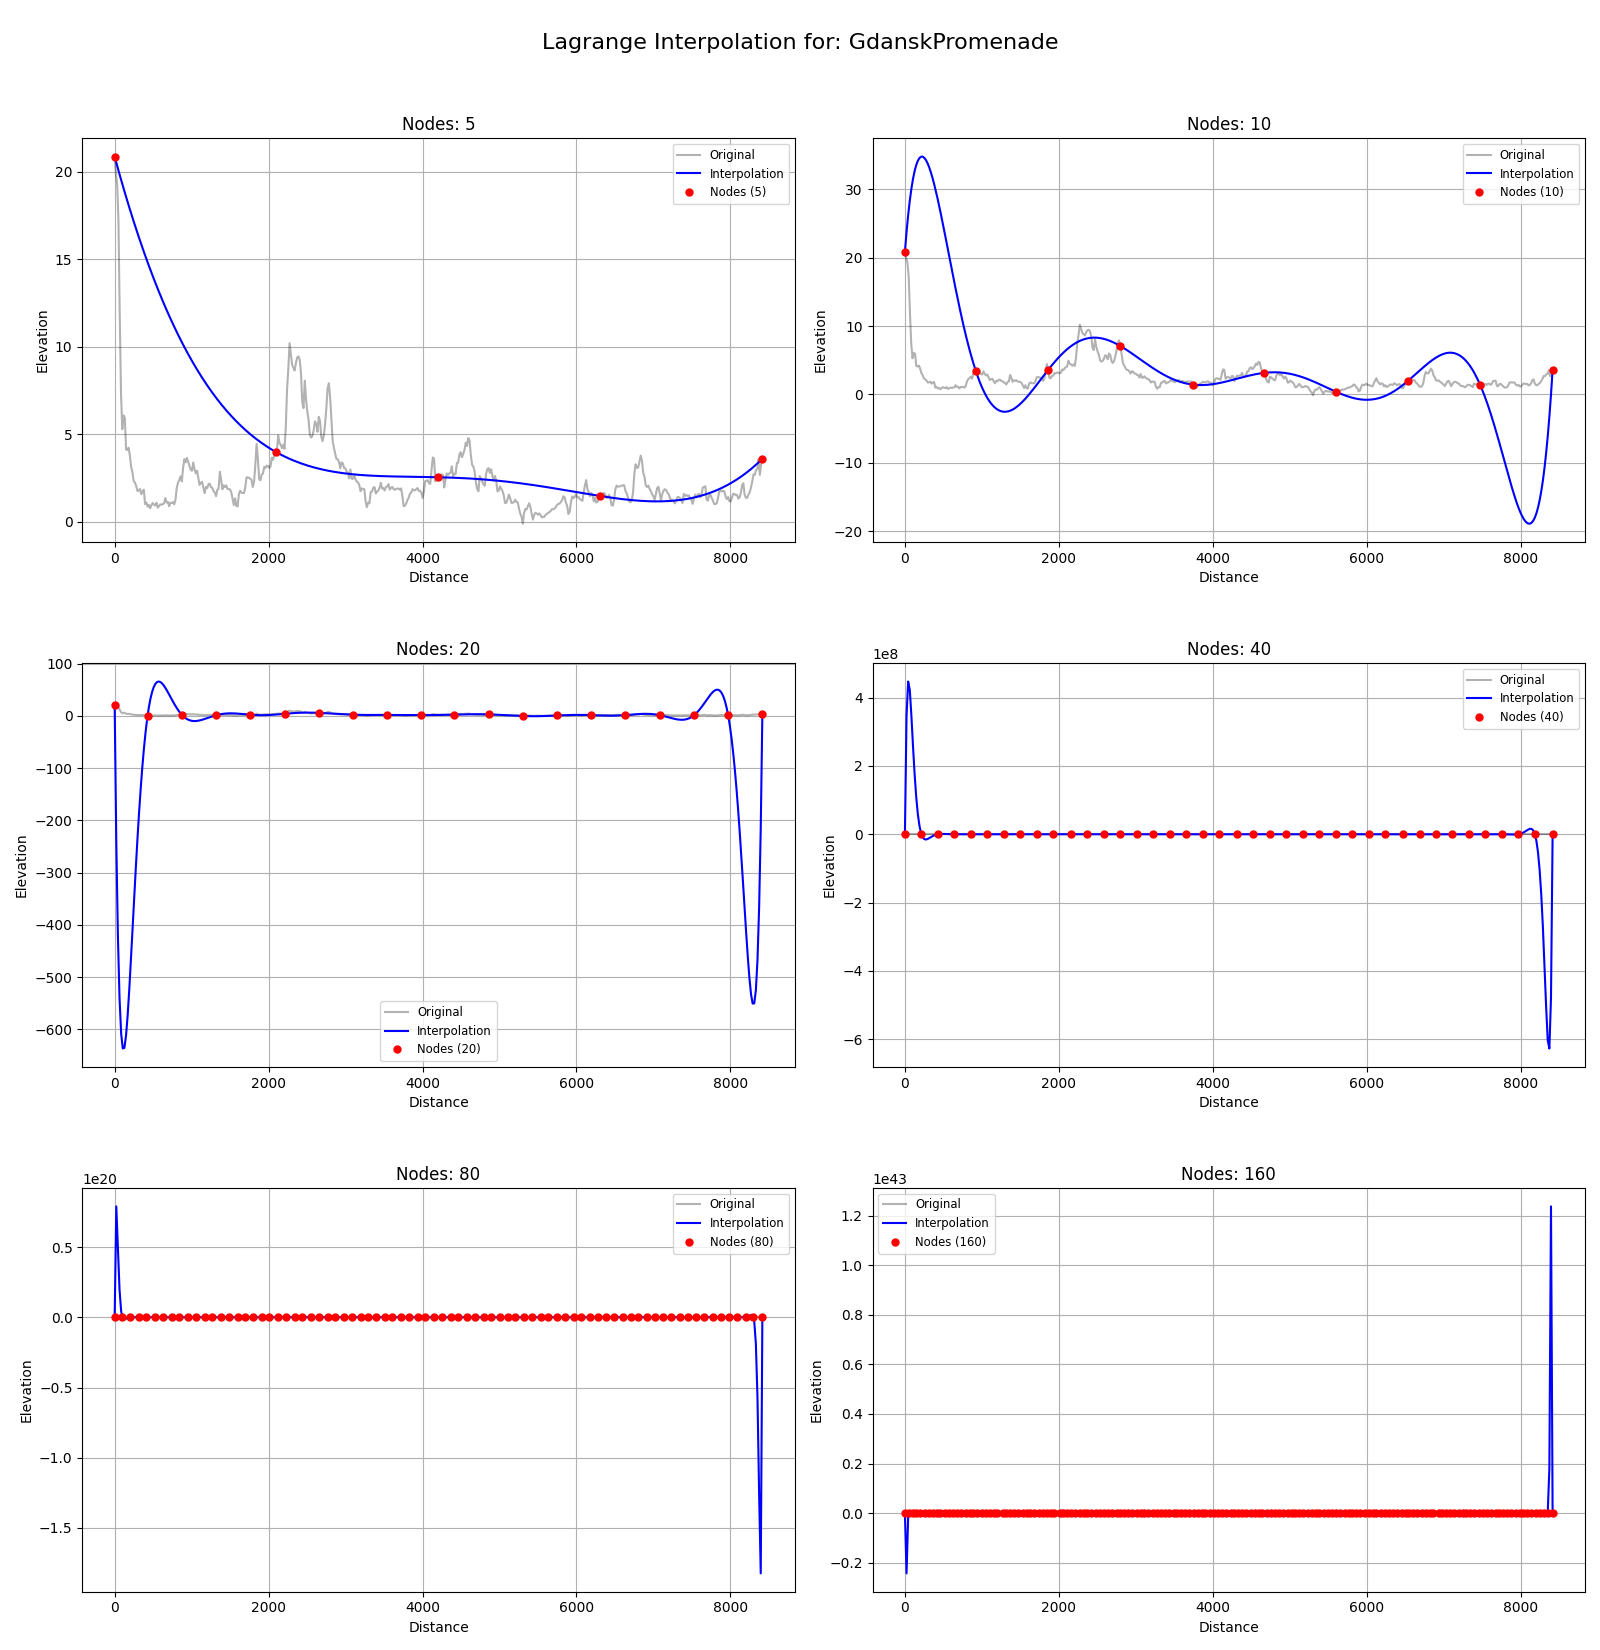
\includegraphics[width=0.8\textwidth]{plots/GdanskPromenade_Lagrange_basic.png}
    \caption{Interpolacja Lagrange'a dla trasy GdanskPromenade (różne liczby węzłów)}
    \label{fig:promenade_lagrange}
\end{figure}
\textbf{Interpretacja (Rysunek \ref{fig:promenade_lagrange}):} 
\begin{itemize}
    \item \textbf{5 węzły:} Interpolacja przebiega gładko, dobrze odwzorowując profil.
    \item \textbf{10 węzłów:} Profil pozostaje gładki, bez widocznych oscylacji.
    \item \textbf{20 węzłów:} Pojawiają się niewielkie oscylacje na końcach przedziału.
    \item \textbf{40 węzły:} Oscylacje na krańcach są wyraźniejsze, dokładność w środku dobra.
    \item \textbf{80 węzły:} Silne oscylacje na końcach, pogorszenie jakości interpolacji.
    \item \textbf{160 węzłów:} Bardzo duże oscylacje na krańcach, interpolacja niestabilna.
\end{itemize}

\subsection{Trasa: Hel}
\begin{figure}[H]
    \centering
    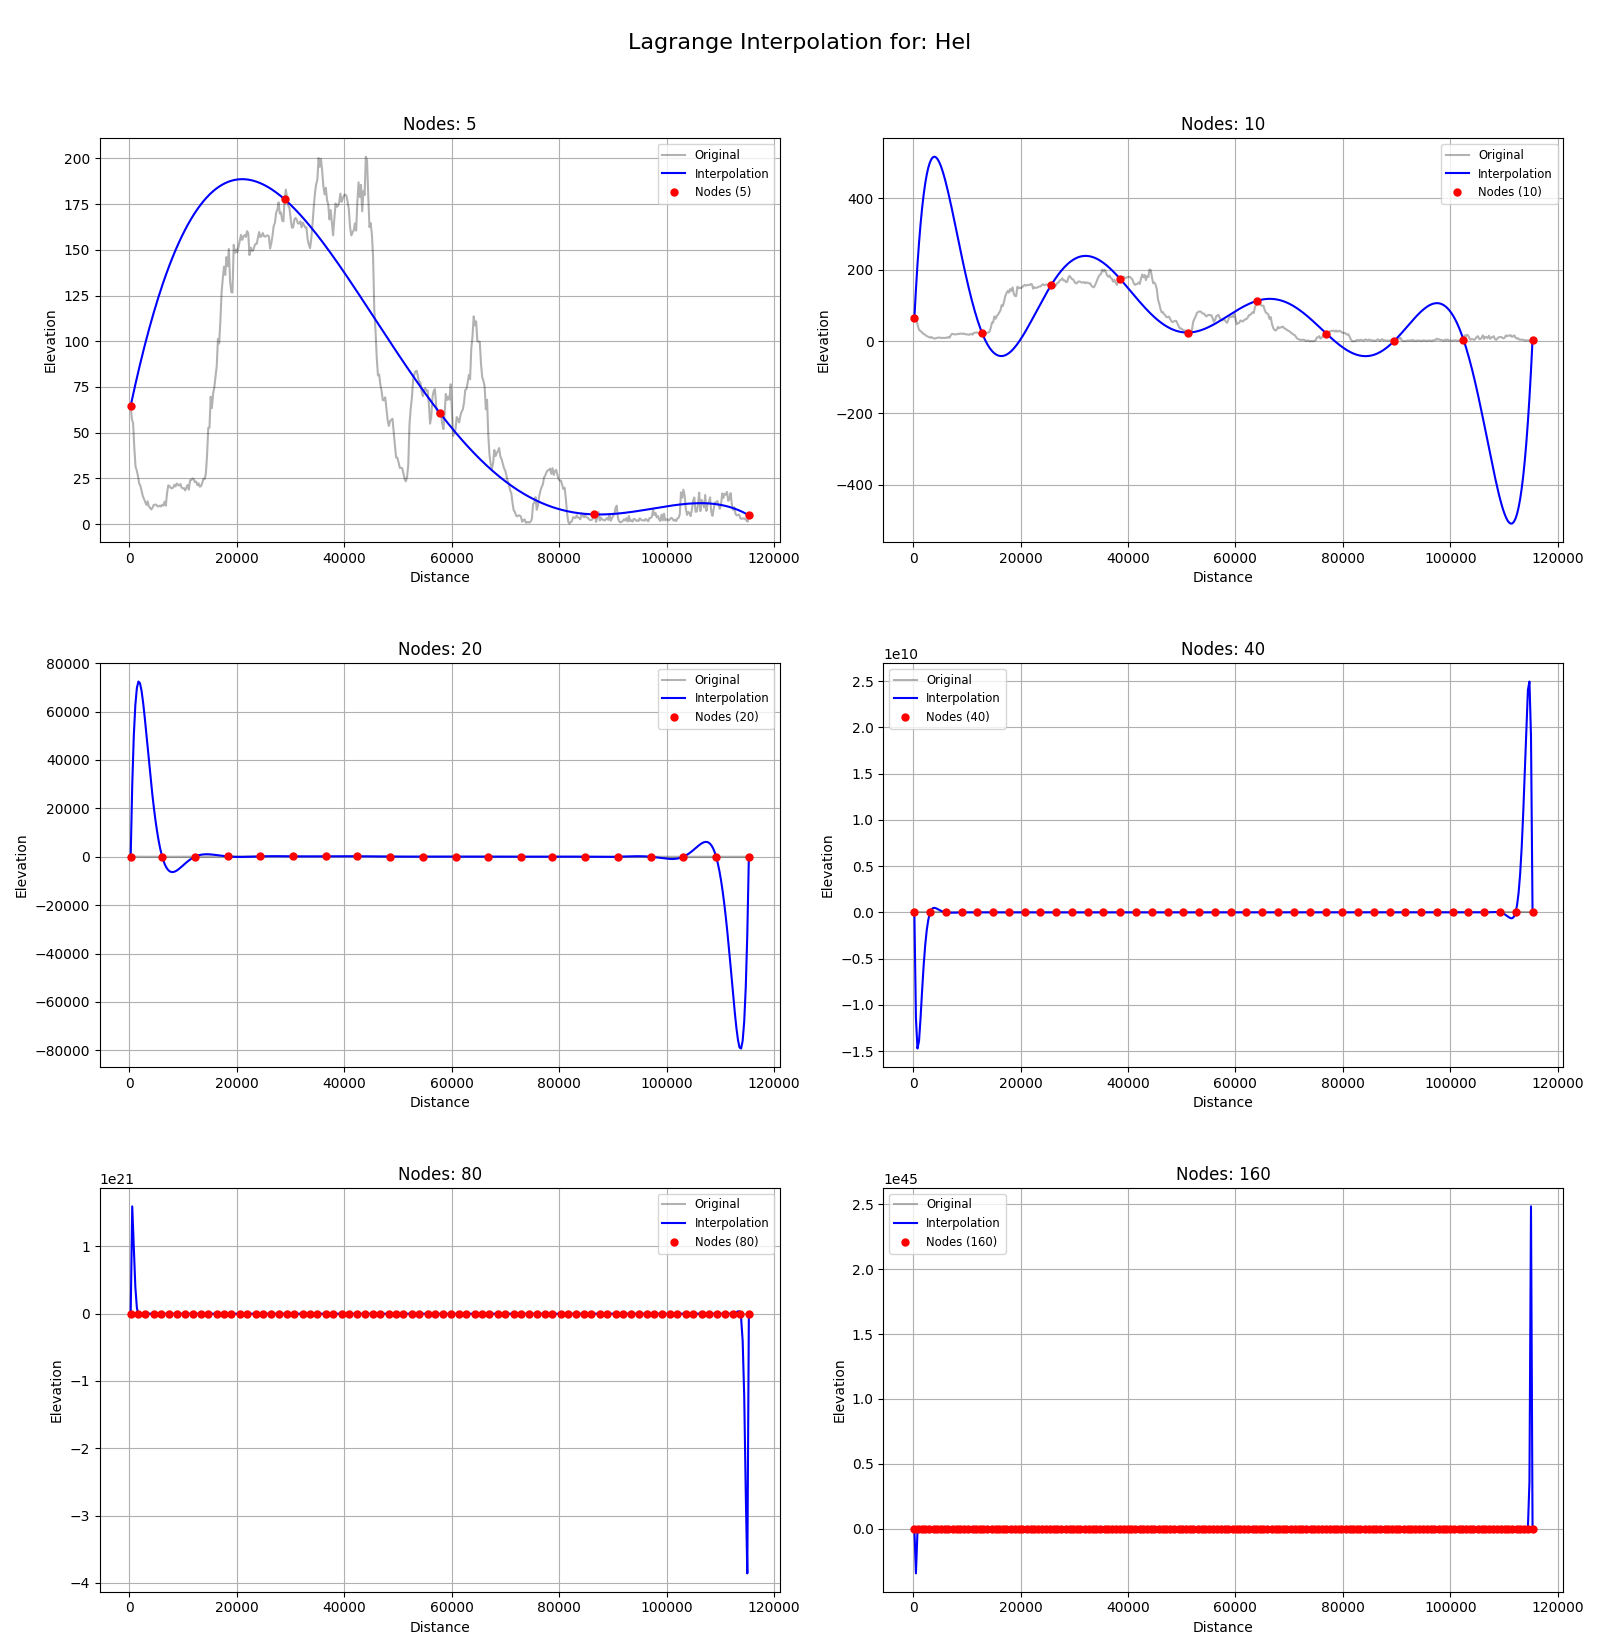
\includegraphics[width=0.8\textwidth]{plots/Hel_Lagrange_basic.png}
    \caption{Interpolacja Lagrange'a dla trasy Hel (różne liczby węzłów)}
    \label{fig:hel_lagrange}
\end{figure}
\textbf{Interpretacja (Rysunek \ref{fig:hel_lagrange}):} 
\begin{itemize}
    \item \textbf{5 węzły:} Profil odwzorowany poprawnie, bez zakłóceń.
    \item \textbf{10 węzłów:} Nadal brak istotnych oscylacji, dobra zgodność z danymi.
    \item \textbf{20 węzły:} Pojawiają się lekkie oscylacje na końcach.
    \item \textbf{40 węzły:} Oscylacje na krańcach są już widoczne.
    \item \textbf{80 węzły:} Oscylacje wyraźnie zaburzają przebieg na końcach.
    \item \textbf{160 węzły:} Bardzo silne oscylacje, interpolacja traci sens fizyczny.
\end{itemize}

\section{Analiza podstawowa interpolacji funkcjami sklejanymi}
\subsection{Trasa: GdanskPromenade}
\begin{figure}[H]
    \centering
    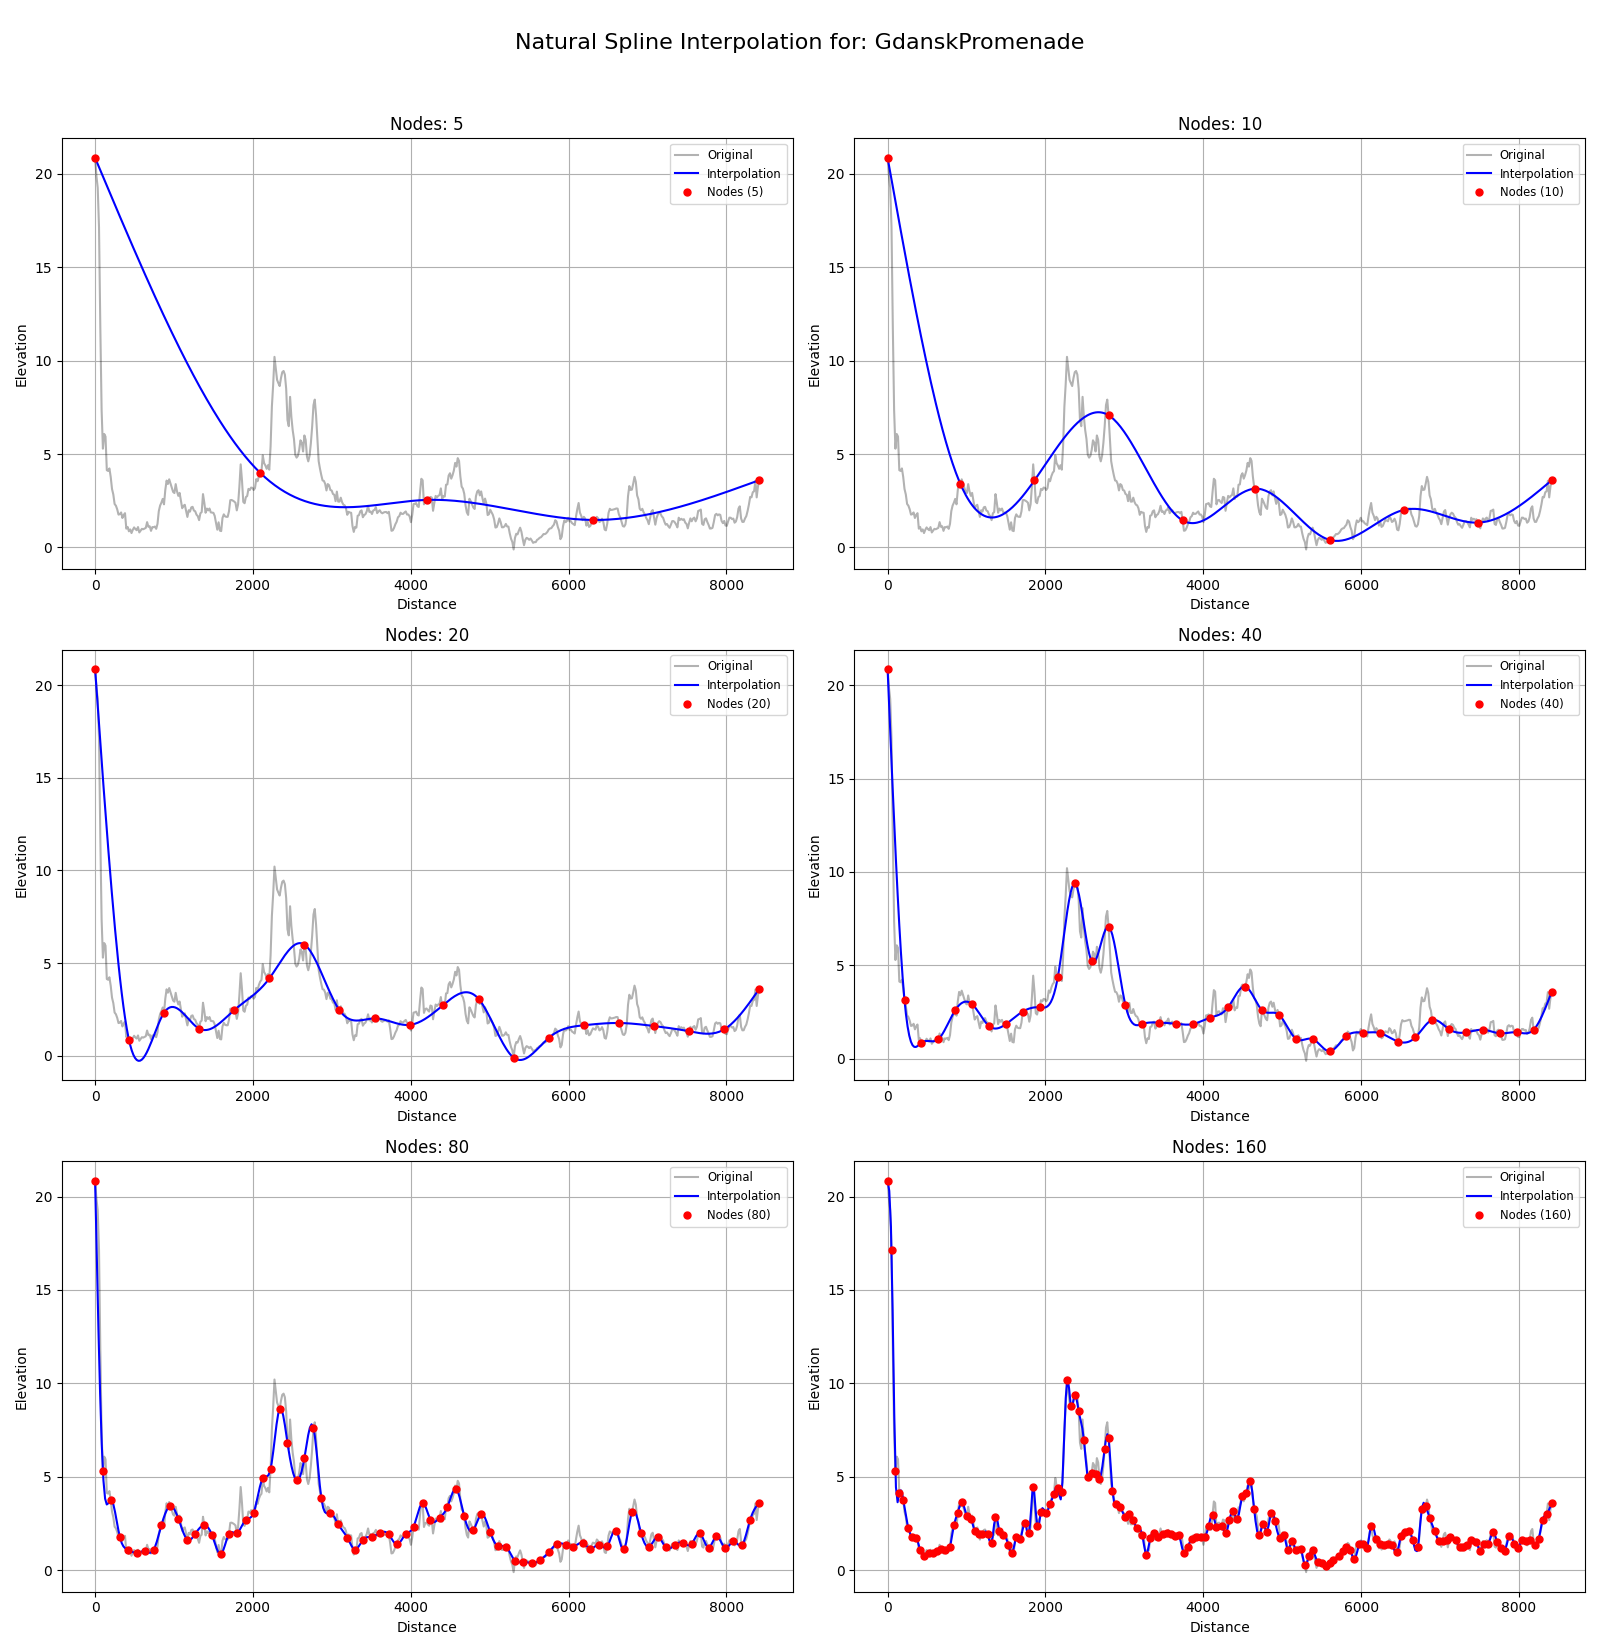
\includegraphics[width=0.8\textwidth]{plots/GdanskPromenade_Spline_basic.png}
    \caption{Interpolacja splajnami kubicznymi dla trasy GdanskPromenade (różne liczby węzłów)}
    \label{fig:promenade_splajny}
\end{figure}
\textbf{Interpretacja (Rysunek \ref{fig:promenade_splajny}):} 
\begin{itemize}
    \item \textbf{5 węzły:} Profil gładki, dobrze aproksymowany.
    \item \textbf{10 węzłów:} Bardzo dobra zgodność z danymi, brak oscylacji.
    \item \textbf{20 węzły:} Dokładność rośnie, przebieg pozostaje gładki.
    \item \textbf{40 węzły:} Wysoka jakość aproksymacji, brak artefaktów.
    \item \textbf{80 węzły:} Profil bardzo dobrze odwzorowany, bez zakłóceń.
    \item \textbf{160 węzłów:} Idealne dopasowanie, brak niepożądanych efektów.
\end{itemize}

\subsection{Trasa: Hel}
\begin{figure}[H]
    \centering
    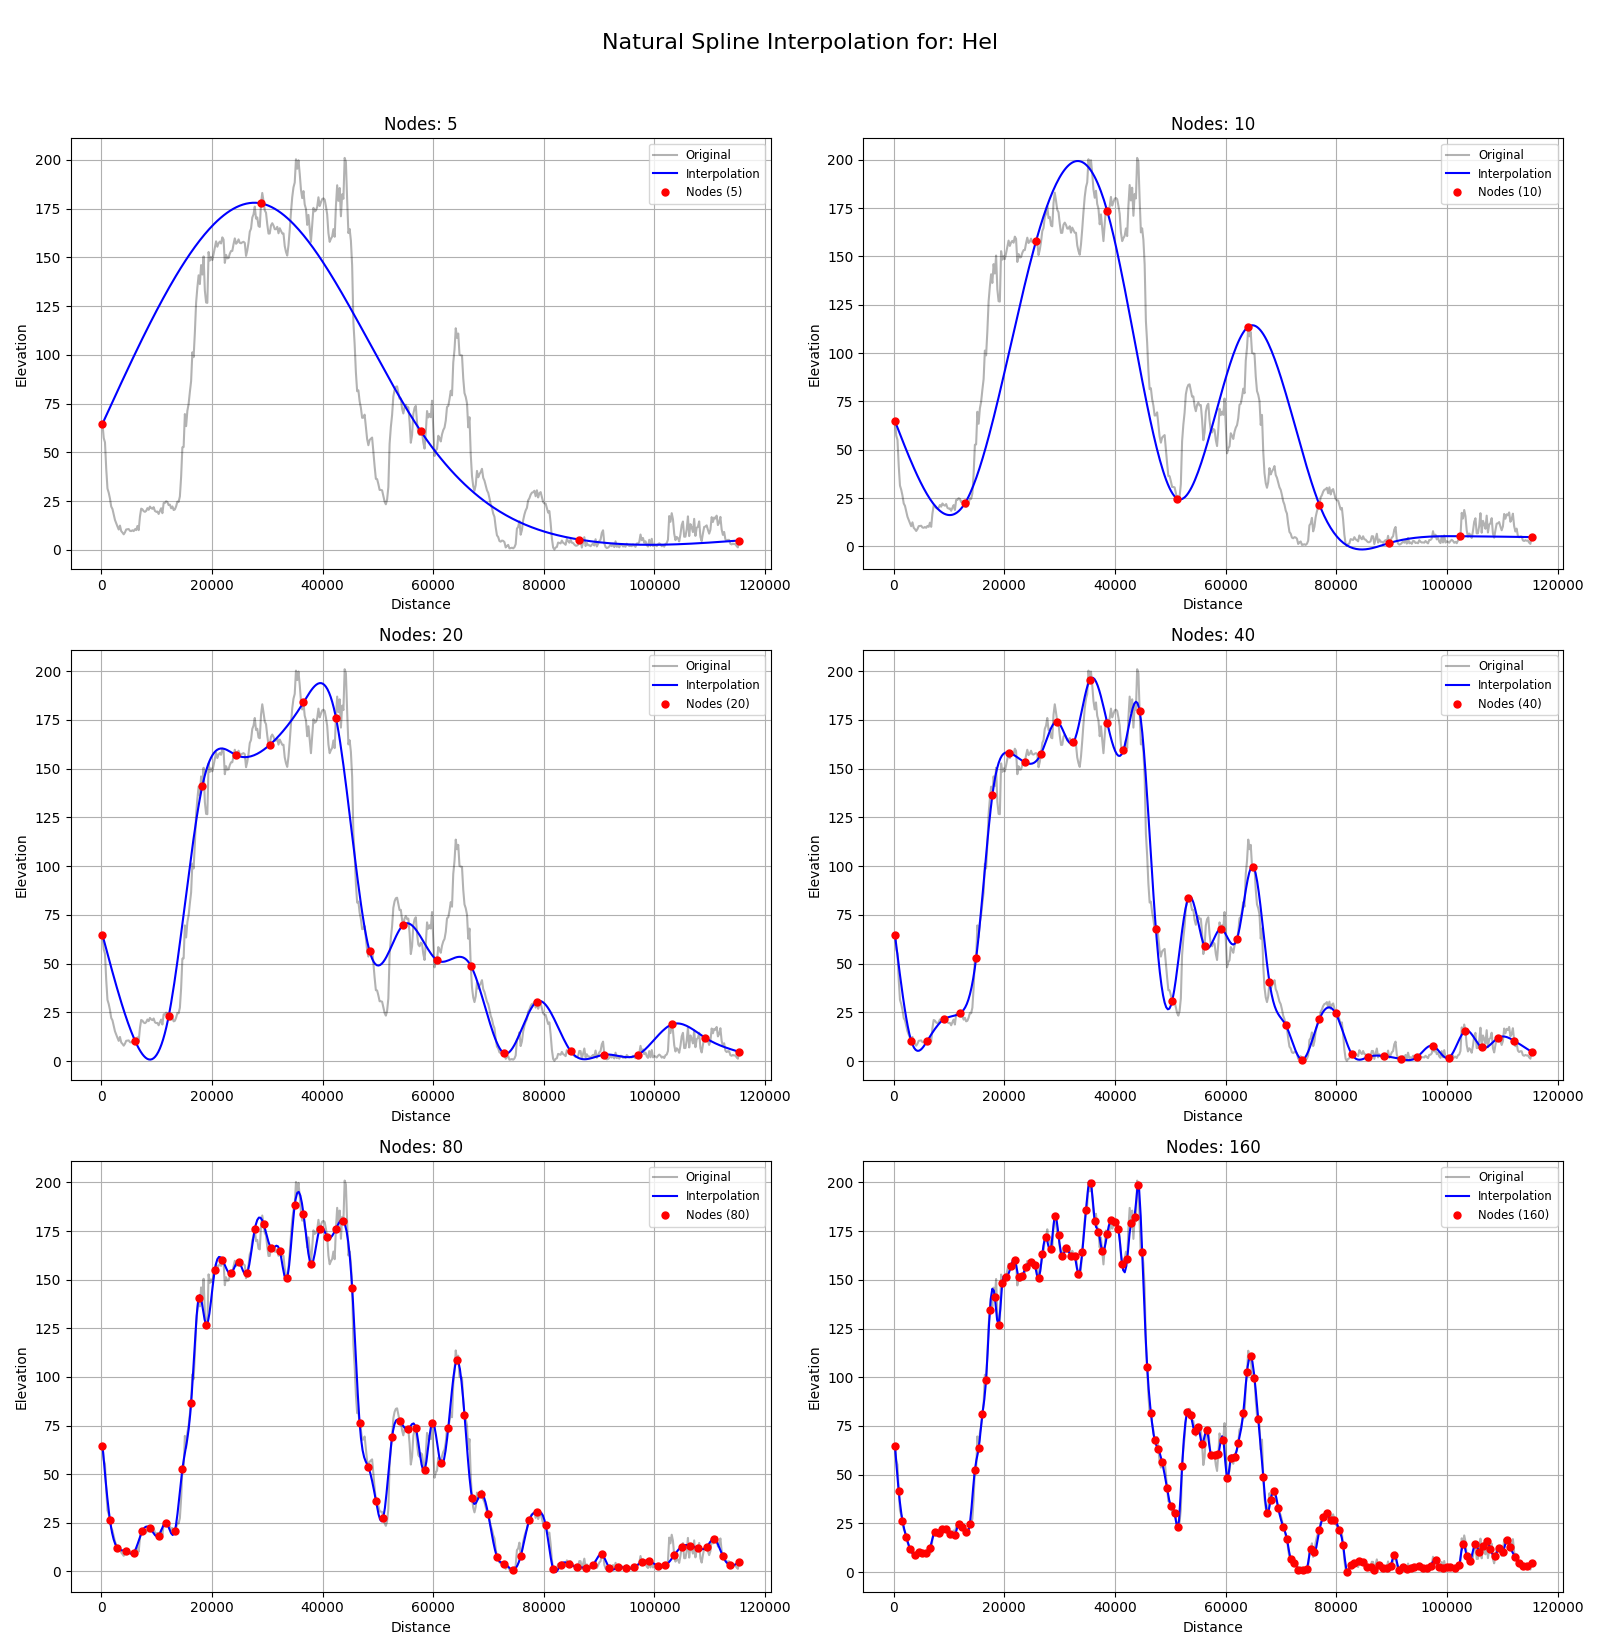
\includegraphics[width=0.8\textwidth]{plots/Hel_Spline_basic.png}
    \caption{Interpolacja splajnami kubicznymi dla trasy Hel (różne liczby węzłów)}
    \label{fig:hej_splajny}
\end{figure}
\textbf{Interpretacja (Rysunek \ref{fig:hej_splajny}):} 
\begin{itemize}
    \item \textbf{5 węzły:} Profil odwzorowany gładko, bez zakłóceń.
    \item \textbf{10 węzłów:} Bardzo dobra zgodność z oryginałem.
    \item \textbf{20 węzły:} Dokładność aproksymacji rośnie, przebieg gładki.
    \item \textbf{40 węzły:} Brak artefaktów, profil bardzo dobrze odwzorowany.
    \item \textbf{80 węzły:} Wysoka jakość aproksymacji, brak oscylacji.
    \item \textbf{160 węzłów:} Idealne dopasowanie do danych.
\end{itemize}

\section{Analiza dodatkowa}
\subsection{Wpływ rozmieszczenia węzłów (węzły Czebyszewa)}
\begin{figure}[H]
    \centering
    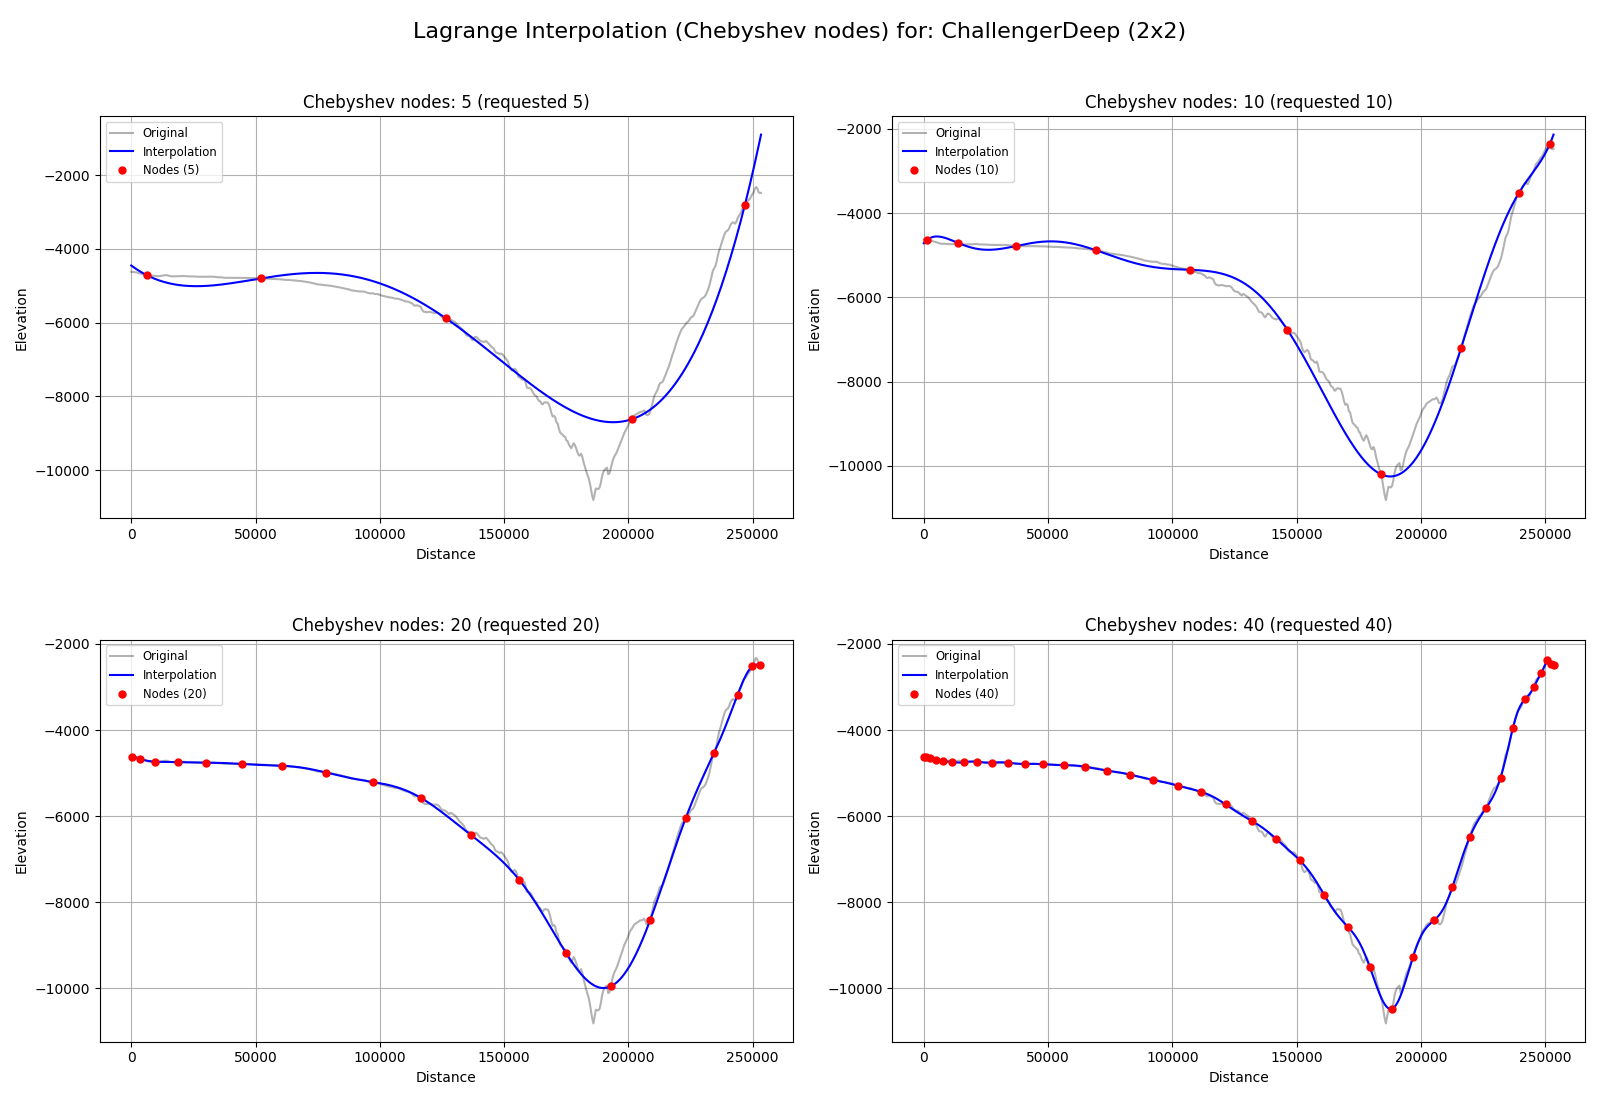
\includegraphics[width=0.8\textwidth]{plots/ChallengerDeep_Lagrange_Chebyshev_2x2.png}
    \caption{Interpolacja Lagrange'a z węzłami Czebyszewa dla trasy ChallengerDeep}
    \label{fig:challengerdeep_chebyshev}
\end{figure}
\textbf{Interpretacja (Rysunek \ref{fig:challengerdeep_chebyshev}):} 
\begin{itemize}
    \item \textbf{5 węzły:} Profil odwzorowany poprawnie, bez oscylacji.
    \item \textbf{10 węzłów:} Dobra zgodność, brak widocznych zakłóceń.
    \item \textbf{20 węzły:} Profil pozostaje stabilny, bez efektu Rungego.
    \item \textbf{40 węzły:} Brak oscylacji, interpolacja stabilna.
    \item \textbf{80 węzły:} Wysoka jakość aproksymacji, brak artefaktów.
    \item \textbf{160 węzłów:} Profil odwzorowany bardzo dobrze, bez niepożądanych efektów.
\end{itemize}

\subsection{Trasa o wielu wzniesieniach}
\begin{figure}[H]
    \centering
    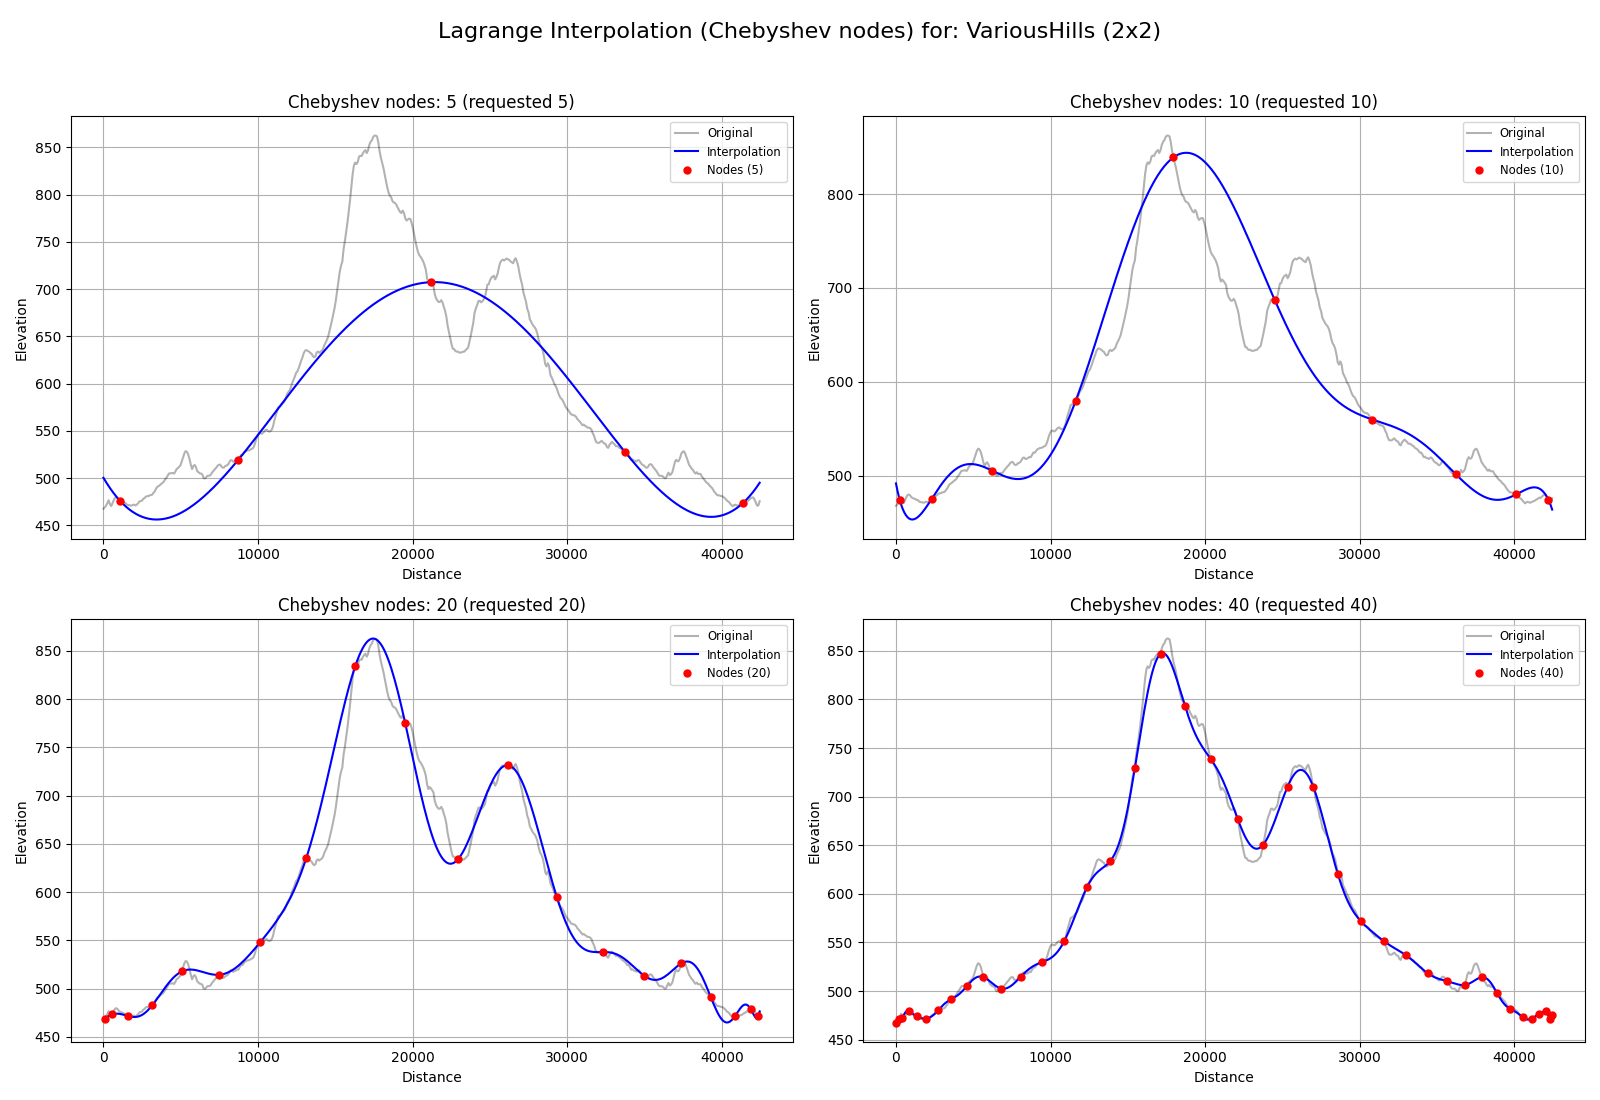
\includegraphics[width=0.8\textwidth]{plots/VariousHills_Lagrange_Chebyshev_2x2.png}
    \caption{Interpolacja Lagrange'a z węzłami Czebyszewa dla trasy VariousHills}
    \label{fig:wiele_wzniesien}
\end{figure}
\textbf{Interpretacja (Rysunek \ref{fig:wiele_wzniesien}):} 
\begin{itemize}
    \item \textbf{5 węzły:} Profil odwzorowany poprawnie, bez zakłóceń.
    \item \textbf{10 węzłów:} Dobra zgodność, brak oscylacji.
    \item \textbf{20 węzły:} Interpolacja stabilna, przebieg gładki.
    \item \textbf{40 węzły:} Brak efektu Rungego, profil dobrze odwzorowany.
    \item \textbf{80 węzły:} Wysoka jakość aproksymacji, brak artefaktów.
    \item \textbf{160 węzłów:} Profil bardzo dobrze dopasowany, bez niepożądanych efektów.
\end{itemize}

\newpage
\section{Interpretacja wyników}
\begin{itemize}
    \item Zwiększanie liczby węzłów w interpolacji Lagrange'a prowadzi do poprawy dokładności tylko do pewnego momentu; dla dużej liczby węzłów pojawia się efekt Rungego (oscylacje na krańcach przedziału).
    \item Rozmieszczenie węzłów według Czebyszewa poprawia stabilność interpolacji wielomianowej.
    \item Interpolacja splajnami kubicznymi jest stabilna nawet dla większej liczby węzłów i dobrze odwzorowuje przebieg trasy.
    \item Charakter trasy (liczba i stromość wzniesień) wpływa na trudność interpolacji -- trasy o gwałtownych zmianach wysokości są trudniejsze do aproksymacji.
\end{itemize}

\section{Podsumowanie}
\label{sec:podsumowanie}
\textbf{Interpolacja wielomianem Lagrange'a} okazała się metodą wrażliwą na liczbę i rozmieszczenie węzłów. Przy większej liczbie równoodległych węzłów (16 i więcej) pojawia się zjawisko Rungego, prowadzące do znacznych oscylacji i zniekształceń profilu. Metoda ta może być stosowana przy niewielkiej liczbie węzłów oraz dla gładkich profili, jednak jej praktyczna użyteczność jest ograniczona. Przeskalowanie dziedziny poprawia stabilność numeryczną, lecz nie eliminuje problemu oscylacji. Wykorzystanie węzłów Czebyszewa (patrz Sekcja \ref{sec:analiza_dodatkowa}) pozwala ograniczyć te efekty i poprawić wyniki, jednak interpolacja wielomianowa pozostaje mniej stabilna i mniej gładka niż funkcje sklejane.

\textbf{Interpolacja naturalnymi funkcjami sklejanymi trzeciego stopnia} wykazała się dużą stabilnością i wysoką jakością aproksymacji. Metoda ta zapewnia gładkie i realistyczne odwzorowanie profilu, niezależnie od liczby węzłów (w testowanym zakresie od 4 do 128). Wraz ze wzrostem liczby węzłów dokładność aproksymacji systematycznie się poprawia, bez pojawiania się niepożądanych artefaktów. Funkcje sklejane dobrze radzą sobie zarówno z profilami gładkimi, jak i bardziej złożonymi.
\vspace{1em}

Podsumowując działanie zaimplementowanych algorytmów:
\begin{itemize}
    \item Implementacja \textbf{interpolacji Lagrange'a} poprawnie odzwierciedla jej właściwości teoretyczne, w tym podatność na zjawisko Rungego przy węzłach równoodległych oraz poprawę stabilności przy \textbf{węzłach Czebyszewa}. W praktyce jej zastosowanie do aproksymacji profilu wysokościowego jest ograniczone.
    \item Implementacja \textbf{naturalnych funkcji sklejanych trzeciego stopnia} działa stabilnie i skutecznie realizuje zadanie aproksymacji profilu.
\end{itemize}

Do aproksymacji profili wysokościowych rekomendowana jest interpolacja funkcjami sklejanymi trzeciego stopnia, ze względu na jej stabilność, gładkość wyników i odporność na problemy charakterystyczne dla interpolacji wielomianowej wysokiego stopnia. Interpolację Lagrange'a, nawet z węzłami Czebyszewa, należy stosować ostrożnie, mając na uwadze możliwość wystąpienia oscylacji.

\end{document}
